\subsection{Principes van cryptografie}
Cryptografische technieken staan een zender toe om data te vermommen zodat een indringer geen informatie kan inwinnen van de onderschepte data. De ontvanger moet natuurlijk in staat zijn om het originele bericht te herstellen.

\noindent Cryptografie wordt gebruikt om boodschappen \textcolor{red}{(\textbf{plain text})} te versleutelen \textcolor{red}{(\textbf{ciphertext})} met een \textcolor{red}{\textbf{crypteringsalgoritme}} zodat ze onleesbaar zijn voor derden.

\begin{figure}[h]
    \centering
    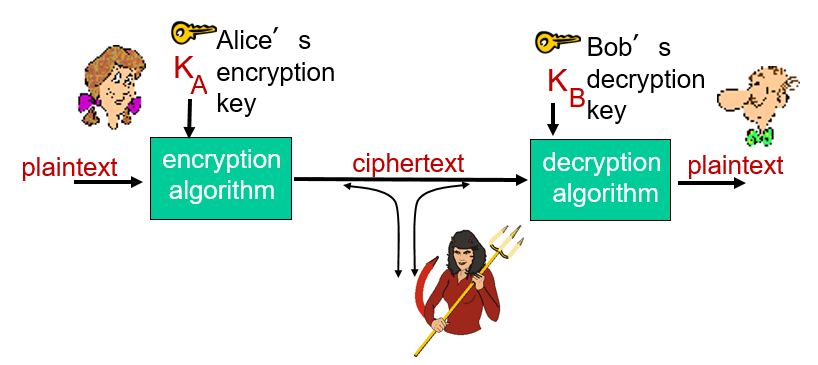
\includegraphics[width=7in]{./img/imghfdst8/hfdst8puntje2.png}\\[1cm]
    \caption{Principes van cryptografie }      
    \label{fig:Principes van cryptografie }
\end{figure}

\noindent \textcolor{red}{\textbf{Leesbare tekst (cleartext)}} is een bericht in zijn originele vorm. De verzender encrypteerd zijn leesbare tekst door gebruik te maken van een encryptie algoritme zodat het geëncrypteerde bericht \textcolor{red}{(\textbf{ciphertext})} onverstaanbaar lijkt voor elke indringer. 

De zender voorziet een \textcolor{red}{\textbf{sleutel (key) $K_A$}}, een string van getallen of tekens, als invoer voor het encryptie algoritme. Het algoritme neemt de sleutel en de leesbare tekst als invoer, en creëert \textcolor{red}{\textbf{ciphertext}} als uitvoer.

De notatie \textcolor{red}{$K_A (m)$} refereert naar de ciphertext vorm van de leesbare tekst. Het eigenlijke encryptie algoritme dat de sleutel \textcolor{red}{$K_A $} gebruikt, blijkt uit de context.
Op dezelfde manier zal de ontvanger een sleutel $K_B$ voorzien, naar het decryptie algoritme dat de \textbf{ciphertext} en de sleutel van de ontvanger gebruikt als invoer, en creëert de originele tekst als uitvoer.
Dat is,als de ontvanger het geëncrypteerde bericht $K_A (m) $ ontvangt en decrypteert door het berekenen van \textcolor{red}{$K_B$($K_A$(m)) = m}.

In symmetrische sleutel systemen, zijn de sleutels van de zender en ontvanger gelijk en geheim.
In publieke sleutel systemen, wordt een sleutel paar gebruikt. Een van de sleutels is gekend door iedereen. De andere is enkel gekend door één persoon.

\subsubsection{Symmetrische sleutel cryptografie}

\begin{figure}[h]
    \centering
    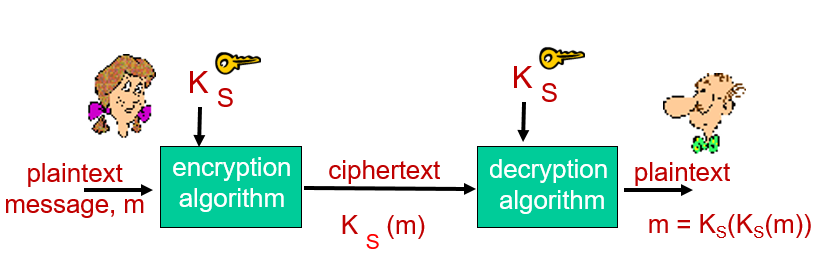
\includegraphics[width=7in]{./img/imghfdst8/hfdst8puntje3.png}\\[1cm]
    \caption{Symmetrische sleutel cryptografie }      
    \label{fig:Symmetrische sleutel cryptografie }
\end{figure}


Hierbij is het belangrijk dat de verzender en ontvanger dezelfde geheime sleutel kennen.
Alle cryptografische algoritmes betrekken het vervangen van een ding naar iets anders.
Voorbeelden van algoritmes:
\begin{itemize}
    \item \textcolor{red}{\textbf{Caesar cipher}}: elke letter vervangen door x-aantal letters verder te gaan in het alfabet. Als men het algoritme kent, kan men het snel kraken. Er zijn maar 25 mogelijkheden.
    \item \textcolor{red}{\textbf{Monoalphabetic cipher}}: verbetering van de Caesar cipher. Enkel wordt een letter vervanger door eender welke andere letter, zo lang als enkel letter een unieke vervangingsletter heeft. Hier zijn er $10^{26}$ mogelijkheden, en zal dus vrij lang duren om te kraken. Maar door gebruik te maken van statistische analyse kan men al een groot deel ontcijferen. Wanneer de indringer enige kennis heeft over de boodschap (woorden die er zeker in voorkomen), blijven er minder sleutel paren over.
    \item \textcolor{red}{\textbf{Polyalphabetic encryption}}: verbetering van de monoalphabetic cipher. Maakt gebruik van meerdere monoalphabetic ciphers, met een specifieke cipher om een letter te coderen in een bepaalde positie.
\end{itemize}

\clearpage

\subsubsubsection{3 soorten aanvallen die een indringer kan uitvoeren}

\begin{enumerate}

\item \textit{Een aanval met alleen versleutelde tekst (=ciphertext only attack)}: De indringer beschikt alleen over de onderschepte versleutelde tekst (=\textbf{ciphertext}).
    \begin{enumerate}
\item 2 benaderingen
        \begin{enumerate}
\item bruteforce: door alle keys te zoeken
\item statistische analyse
        \end{enumerate}

    \end{enumerate}
\item \textit{Een aanval met een bekende onversleutelde tekst}: De indringer weet een beetje waarover de tekst gaat. (Er komt sowieso ‘Alice’ en ‘Bob’ in voor.)
\item \textit{Een aanval met een specifieke onversleutelde tekst}: Hierbij kan de indringer zelf het onversleutelde bericht (=ciphertext) kiezen en daarvan de geëncrypteerde tekst (=chosen plaintext) krijgen.
\end{enumerate}
In gedachte nemend hoe gemakkelijk het kan zijn om een encryptie schema te ontcijferen, kan men drie verschillende scenario’s onderscheiden, afhankelijk van welke info de indringer heeft:
\begin{itemize}
    \item \textbf{Cyphertext-only attack}: de indringer heeft enkel toegang tot de ciphertext en geen zekere informatie over de mogelijke inhoud. Hier kan statistische analyse helpen.
    \item \textbf{Know-plaintext attack}: de indringer heeft weet van bepaalde inhoud, en heeft hierdoor al bepaalde sleutelparen gevonden.
    \item \textbf{Chosen-plaintext attack}: Als de indringer een bepaald bericht kan laten sturen, kan de indringer het encryptie schema ontrafelen.
\end{itemize}

\subsubsubsection{DES = Data Encryption Standard}

\bi
\itf 56-bit symmetric key, 64-bit plaintext input
\itf block cipher with cipher block chaining
\itf how secure is DES?
    \bi
    \itf DES Challenge: 56-bit-key-encrypted phrase decrypted (brute force) in less than a day
    \itf no known good analytic attack
    \ei
\itf making DES more secure:
    \bi
    \itf 3DES: encrypt 3 times with 3 different keys
    \ei
\ei

\subsubsubsection{Block Ciphers}

Wordt gebruikt in veel beveiligde internet protocollen zoals:

\bi
\itf \textcolor{red}{\textbf{PGP}} : voor beveiligde e-mail
\itf \textcolor{red}{\textbf{SSL}} : voor beveiligde TCP connecties
\itf \textcolor{red}{\textbf{IPsec}} : voor beveiligde netwerk-laag transport
\ei

	
\noindent In een \textbf{block cipher}, wordt het bericht dat geëncrypteerd moet worden verwerkt in blokken van x-aantal bits en elk blok wordt onafhankelijk van elkaar geëncrypteerd. Om een blok te coderen, maakt de cipher gebruik van een één op één mapping om de x-bit blok van cleartext naar een x-bit blok van ciphertext in kaart te brengen. Er zijn dus $2^X$ invoer mogelijkheden. Deze $2^X$ invoer kan gepermuteerd worden in $2^X$! verschillende mapping mogelijkheden. We kunnen elk van deze mappings zien als sleutel.

\noindent Hoewel een volledige lijst van block ciphers, met gematigde waardes van x een robuust symmetrische sleutel encryptie schema kan produceren, zijn ze ontzettend moeilijk om te implementeren. Voor x = 64 moeten de zender en ontvanger een lijst onderhouden met $2^64$ invoer waardes, wat een onhaalbare taak is. Bovendien, als de zender en ontvanger van sleutel zou veranderen, moeten ze elk een tabel genereren. Daarom zal men deze manier niet gebruiken.
In plaats daarvan, gaan block ciphers typisch meestal gebruiken maken van functies die willekeurig gepermuteerde tabellen simuleren.

\noindent (Voorbeeld van zo’n functie met k = 64 bits.) De functie deelt eerst een 64 block in 8 delen die 8 bits bevatten. Elke deeltje wordt verwerkt door een 8 bit op 8 bit tabel, die beheerbaar is in grote. Vervolgens worden de 8 deeltjes weer in elkaar gezet in een 64 bit blok. De posities van de 64 bits in het blok worden dan door elkaar gegooid om een 64 bit uitvoer te verkrijgen die dan weer dient voor de input van een 64 bit blok zodat de cyclus opnieuw uitgevoerd kan worden. Na n-aantal keren, geeft de functie een 64-bit block van ciphertext. De bedoeling van de rondes is om elke invoer bit een andere output te hebben.

\noindent Er zijn vandaag verschillende populaire block ciphers zoals DES, 3DES en AES. Gebruiken elk functies in plaats van voorgedefinieerde tabellen.
\begin{itemize}
\item \textbf{DES (Data Encryption Standard)}: maakt gebruik van 64 bit blokken met een 56 bit sleutel. Maar dit is niet zo veilig want dit kan binnen een dag gekraakt worden.
\item \textbf{3DES}: DES veiliger maken om het 3 keer te encrypteren met 3 verschillende sleutels.
\item \textbf{AES (Advanced Encryption Standard): }gebruikt 128 bit blokken en kan werken met sleutels die 128, 192 en 256 bits lang zijn.

\end{itemize}


\subsubsubsection{Cipher-Block koppelen}

$\rightarrow$ Een techniek die gebruikt wordt om encryptie toe te passen bij berichten die verzonden worden.

\noindent Als we gebruik maken van een block cipher door gewoon het bericht te splitsen in x-bit blokken en onafhankelijk van elkaar encrypteren, treedt er een subtiel maar belangrijk probleem op. Twee of meerdere clear-text blokken kunnen identiek zijn. Voor deze identieke blokken, zal de block cipher dezelfde ciphertext maken. Een aanvaller kan potentieel naar de cleartext gokken wanneer hij identieke blokken ziet, en zo zelfs het hele bericht ontcijferen.

Om dit probleem op te lossen, kunnen we wat willekeur inbrengen in de ciphertext. Hiervoor wordt een techniek gebruikt die de \textcolor{red}{\textbf{Cipher Block Chaining (CBC)}} genoemd wordt. Het idee is om enkel één willekeurige waarde mee te sturen met het eerste bericht en dat de zender en ontvanger de CBC gebruiken. Dit gaat als volgt te werk:

\begin{itemize}

\item Voor het encrypteren van de data, genereert de zender een willekeurig x-bit string, de Initialisatie Vector (IV) genoemd. Deze wordt in cleartext verzonden naar de ontvanger.

\item Voor het eerste blok berekent de zender m(1) + c(0), daarna berekent het de \textbf{XOR} van het eerste blok met de \textbf{IV} en hierdoor krijgt men \textcolor{red}{c(1) = $K_S(m(1) + c(0))$}. C(1) wordt verstuurd naar de ontvanger.

\item Voor het i-de blok, genereert de zender de i-de ciphertext blok van c(i) = $K_S(m(i) + c(i-1))$.

\end{itemize}

\subsubsubsection{AES: Advanced Encryption Standard}
\bi
\itf symmetric-key NIST standard, replaced DES
\itf Verdeelt data in blokken van 128 bit
\itf Keys van 128, 192 of 256 bit grootte
\itf Als men 1 seconde op DES rekent om een key te decrypteren met bruteforce, duurt het 149 triljoen jaar voor AES om 1 key te decrypteren
\ei


\subsubsection{Publieke sleutel encryptie}

\subsubsubsection{Diffie-Hellman key echange algoritm}
\begin{figure}[h]
    \centering
    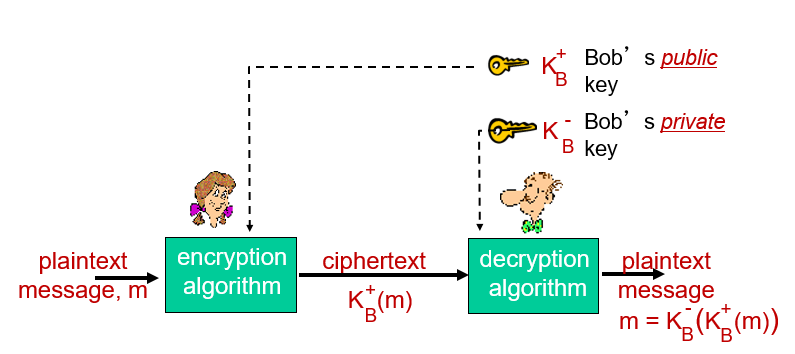
\includegraphics[width=7in]{./img/imghfdst8/hfdst8puntje5.png}\\[1cm]
    \caption{Diffie-Hellman key echange algoritm }      
    \label{fig:Diffie-Hellman key echange algoritm }
\end{figure}

\noindent aantal vereisten nodig:

\be
\itf De ontvanger heeft 2 sleutels:
    \be
    \itf een publieke sleutel $(K^+_B)$ die beschikbaar is voor iedereen en door de zender gebruikt wordt om het bestand te encrypteren
    \itf een privé sleutel $(K^-_B)$ die enkel de ontvanger kent en gebruikt wordt om het ontvangen bestand te decrypteren
   \itf zodat $(K^-_B)$($(K^+_B)$(m)) = m
    \ee
\itf Gegeven publieke sleutel $(K^+_B)$, zou het onmogelijk moeten zijn om een private sleutel $(K^-_B)$ te genereren
\ee

Maar komen 2 grote zorgen:
\begin{itemize}
\item Een indringer die het bericht onderschept zal enkel brabbeltaal zien, de indringer kent zowel de publieke sleutel als het algoritme gebruikt voor de encryptie. De indringer kan dus een chosen-plaintext attack uitvoeren en zo dus eender welk bericht decoderen. De indringer kan proberen om bepaalde delen van het bericht te decoderen.
\item Sinds de encryptie sleutel van de ontvanger publiek is, kan eender wie een geëncrypteerd bericht sturen naar de ontvanger. Een indringer kan zeggen dat hij stuurt als de zender.

\end{itemize}

\noindent Om deze manier van werken te laten slagen, moet de selectie van de sleutel en encryptie/decryptie gedaan worden op zo’n manier dat het bijna onmogelijk is voor een indringer om de prive sleutel van de ontvanger te bepalen of het bericht kan decrypteren of raden.

\subsubsubsection{RSA}

Maakt uitgebreid gebruik van rekenkundige bewerkingen gebruiken van modulo-n.

X mod n wilt gewoonweg zeggen de rest van x wanneer het gedeeld wordt door n. In modulaire rekenkunde gebruikt men nog de gebruikelijke operaties van toevoeging, vermenigvuldiging en exponentieel. Echter, het resultaat van elke operatie wordt vervangen door de numerieke rest van wat er overschiet wanneer het resultaat gedeeld is door n.
Volgende handeling zijn er:

\begin{itemize}

\item $[(a\ mod\ n)  + (b\ mod\ n)] \ mod\ n\ = (a + b)\ mod\ n$
\item $[(a\ mod\ n) - (b\ mod\ n)] \ mod\ n\ = (a - b)\ mod\ n$
\item $[(a\ mod\ n) * (b\ mod\ n)] \ mod\ n\ = (a * b)\ mod\ n$
\item $(a\ mod\ n)^d = a^d\ mod\ n$
\end{itemize}
Een bericht is niet anders dan een bit patroon die uniek gerepresenteerd kan worden door een integer. Er zijn twee samenhangende onderdelen van RSA:

\begin{itemize}
\item De keuze van de publieke en prive sleutel
\item Het encryptie en decryptie algoritme
\end{itemize}

\subsubsubsection{RSA: (een public/private key pair genereren)}

Om een publieke en prive RSA sleutel te genereren, worden volgende stappen gevolgd:

\begin{enumerate}
\item Er worden eerst 2 grote \textbf{priemgetallen} gekozen, \textbf{p} en \textbf{q}. Hoe groter de waardes hoe moeilijker het is om de RSA te kraken, maar hoe langer het duurt om te coderen en decoderen. p*q < 1024 bits
\item Bereken $n = p*q$ en $z = (p - 1)*(q - 1)$
\item Er wordt een getal \textbf{e} (van encryption) gekozen (<n) dat \textbf{geen factoren gemeenschappelijk} heeft met z.
\item Er wordt een getal \textbf{d} (van decryption) gekozen zodanig dat \textbf{ed – 1} exact deelbaar is door z. $\rightarrow$ \textbf{ed mod z = 1}
\item De publieke sleutel $(K^+_B)$ bestaat uit het paar getallen \textbf{(n,e)}. De privé sleutel $(K^-_B)$ bestaat uit het paar getallen (n,d)
\end{enumerate}

\subsubsubsection{RSA : encryptie en decryptie}

De encryptie wordt op de volgende manier gedaan:

\begin{enumerate}
\item Om een bericht te encrypteren, bereken $c = m^e\ mod\ n$.
\item Om het ontvangen ciphertext bericht \textbf{c} te decrypteren, berekent Bob: $m = c^d\ mod\ n$.
\end{enumerate}

\noindent Dus algemeen: $m = (m^e\ mod\ n)^d \ mod\ n$

\begin{figure}[h]
    \centering
    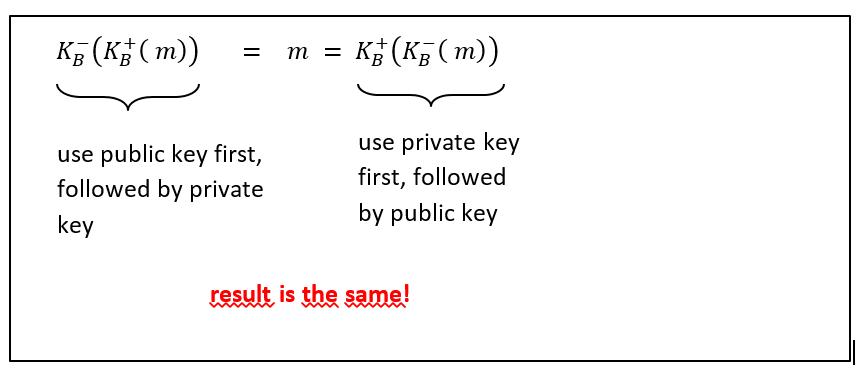
\includegraphics[width=7in]{./img/imghfdst8/diffie.PNG}
    \caption{encryptie en decryptie rsa}      
    \label{fig:encryptie en decryptie rsa }
\end{figure}

\subsubsubsection{Sessie sleutels}

\textcolor{red}{\textbf{Sessiesleutel}:} De gedeelde sleutel die wordt gebruikt om de gegevens zelf te encrypteren.

\bi
\itf Machtsverheffingen voor RSA zijn behoorlijk tijdrovende bezigheden
\itf DES is minimaal 100 keer sneller dan RSA
\ei
RSA wordt vaak gebruikt in combinatie met symmetrische sleutel cryptografie.

Bob en Alice gebruiken RSA om een symmetrische sleutel (=sessiesleutel) $K_S$ uit te wisselen. Eenmaal ze beiden de sleutel Ks hebben, gebruiken ze symmetrische sleutel cryptografie.

De zender moet de ontvanger informeren over de sessie sleutel, omdat deze gedeelde symmetrische sleutel gebruikt gaat worden met een symmetrische sleutel cipher.

De zender encrypt de sessie sleutel door middel van de publieke sleutel van de ontvanger. Dit wordt dan $c = (K_S)^e\ mod\ n$.\\ De ontvanger krijgt de RSA geëncrypteerde sessie sleutel, c en decrypt het om de sessie sleutel de krijgen.

\clearpage

\subsubsubsection{Waarom werkt RSA?}

RSA encryptie/decryptie lijkt eerder magisch. Waarom is het mogelijk bij het toepassen van het encryptie algoritme en daarna het decryptie algoritme, om het originele bericht te herstellen? 
Onder RSA encryptie, een bericht m wordt tot de macht e gedaan modulo-n, dat is $c = m^e\ mod\ n$.
Decryptie wordt uitgevoerd het verhogen van deze waarde tot de macht d en opnieuw modulo n. Het resultaat van een encryptie stap gevolgd door een decryptie stap is dus $(m^e\ mod\ n)^d\ mod\ n$.

Een belangrijke eigenschap van modulo is $(a\ mod\ n)^d\ mod\ n\ = a^d\ mod\ n$ voor elke waarde a, n en d. Dus gebruik makend van de eigenschap $a = m^e$ krijgen we $(m^e\ mod\ n)^d\ mod\ n = m^{ed}\ mod\ n$.

We moeten nog aantonen dat $m^{ed}\ mod\ n = m$. \\\\Om een deel van de magie weg te werken, moeten we een magisch resultaat uit de getal theorie gebruiken. Specifiek, we hebben het resultaat nodig dat zegt dat als p en q priem getallen zijn, $n = pq, $ en $ z = (p – 1)(q – 1)$, dan is $x^y\ mod\ n$ gelijk aan $x^{y}\ mod\ z) \ mod\ n$. Als we dit resultaat toepassen met x = m en y = ed dan krijgen we $m^{ed}\ mod\ n = m^{ed}\ mod\ z) \ mod\ n$.\\\\
Maar herinner dat we e en d zo hebben gekozen dat $ed\ mod\ z = 1$. \\\\Dit geeft ons $m^{ed}\ mod\ n = m^1\ mod\ n = m$. Wat exact het resultaat is dat we zochten. 

We kunnen hierdoor ook zeggen dat $(m^d\ mod\ n)^e\ mod\ n = m^{de}\ mod\ n = m^{ed}\ mod\ n = (m^e\ mod\ n)^d\ mod\ n$

De veiligheid van RSA vertrouwt op het feit dat er geen gekende algoritmes zijn voor het snel vormen van een nummer, in dit geval de publieke waarde n, in priem getallen p en q. Als iemand p en q kende, dan de publieke waarde e, kan men gemakkelijk de geheime sleutel d berekenen.
Aan de andere kant, het is niet bekend of er een algoritme bestaat, dus de veiligheid van RSA is niet gegarandeerd.
